\documentclass[master.tex]{subfiles}
\begin{document}

\chapter{Example Formal System --- Propositional Logic}
\label{chap:example_propositional_logic}

Once you are familiar with some basic features and usability of \emph{Phometa}
from the last chapter. This chapter aims to show more advance features on
another formal system named \emph{Propositional Logic} which is the most well
known logical system\footnote{Logical system is a formal system together with
  semantics\supercite{formal-system-wiki}}.

Logic, in general, works so well with traditional derivation system, hence there
is spacial name called \emph{Natural Deduction} which is a combination of any
kind of Logic together with derivation system.

\section{Grammars}

As usual, the first thing that needed to be defined grammars. Propositional
Logic has 4 grammars which are \pgmr{Prop}, \pgmr{Atom},
\pgmr{Context}, and \pgmr{Judgement} as its grammars.

\pgmr{Prop} is a proposition, semantically, it is a term that can be evaluated
to either true or false (given that there are no meta variables in the term).
Grammars of \pgmr{Prop} can be defined in Phometa as the following

\begin{figure}[H]
    \centering
\begin{minipage}{0.7\textwidth}
    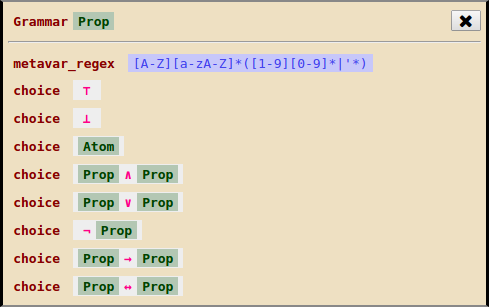
\includegraphics[width=\textwidth]{prop-grammar-prop}
\end{minipage}
\caption{Definition of \pgmr{Prop}}
\label{fig:prop-grammar-prop}
\end{figure}

This grammar is equivalence to the following Backus Normal Form

\begin{figure}[H]
\begin{framed}
\begin{lstlisting}[style=bnf]
<Prop> ::= $\top$ | $\bot$ | <Atom>
         | <Prop> $\wedge$ <Prop>
         | <Prop> $\vee$ <Prop>
         | $\neg$ <Prop>
         | <Prop> $\rightarrow$ <Prop>
         | <Prop> $\leftrightarrow$ <Prop>
         | meta-variables comply with regex
             /[A-Z][a-zA-Z]*([1-9][0-9]*|'*)/
\end{lstlisting}
\end{framed}
\caption{Backus-Naur Form correspond to \pgmr{Prop}}
\label{fig:prop-bnf-prop}
\end{figure}

\newcommand{\propTop}[0]{\bat{\pifmt{$\top$}}}
\newcommand{\propBot}[0]{\bat{\pifmt{$\bot$}}}
\newcommand{\propAnd}[0]{\pifmt{$\wedge$}}
\newcommand{\propOr}[0]{\pifmt{$\vee$}}
\newcommand{\propNot}[0]{\pifmt{$\neg$}}
\newcommand{\propImp}[0]{\pifmt{$\rightarrow$}}
\newcommand{\propIff}[0]{\pifmt{$\leftrightarrow$}}

On the $3^{rd}$ choice of \pgmr{Prop} depends on \pgmr{Atom} which represents
primitive truth statement that cannot be broken down any further. It can be
defined in Phometa as the following.

\begin{figure}[H]
    \centering
\begin{minipage}{0.7\textwidth}
    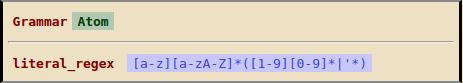
\includegraphics[width=\textwidth]{prop-grammar-atom}
\end{minipage}
\caption{Definition of \pgmr{Atom}}
\label{fig:prop-grammar-atom}
\end{figure}

You can see that \kLiteralRegex\ appears inside \pgmr{Atom} definition, this
allows \pgmr{Atom} be instantiated by literal which is similar to meta variable,
the only different is that literal doesn't have ability to be substituted by
arbitrary term like meta variable.

At this stage, you might wonder that why \pgmr{Prop} needs both of meta
variables and \pgmr{Atom}. Well, meta variable will be used when referring to
something general and \pgmr{Atom} will used when referring to particular truth
statement. For example, if we can prove that \term{prop-term-lem-big-a} is
valid, then terms such as \term{prop-term-lem-top},
\term{prop-term-lem-top-imply-bot}, \term{prop-term-lem-big-b},
\term{prop-term-lem-rainning}, and \term{prop-term-lem-big-b-and-rainning} are
also valid. However, if we can prove that \term{prop-term-lem-rainning} is
valid, we don't want to expose this proof to other terms since it might be
proven from specific knowledge.

Now, we have enough ingredient to create a proper proposition, one might say
that we can start proving it directly, however, most of proposition that we will
dealing with only holds under certain assumptions, hence, a \emph{judgement}
should be in the form $A_1, A_2, ..., A_n \vdash B$ where $A_{1..n}$ are
assumptions and $B$ is conclusion.

To model a judgement in Phometa, first we need to model assumptions or in the
other name, \pgmr{Context} as the following

\begin{figure}[H]
    \centering
\begin{minipage}{0.7\textwidth}
    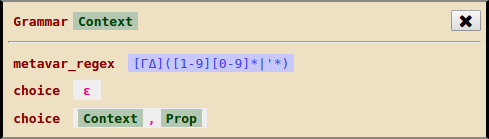
\includegraphics[width=\textwidth]{prop-grammar-context}
\end{minipage}
\caption{Definition of \pgmr{Context}}
\label{fig:prop-grammar-context}
\end{figure}

\newcommand{\propEmptyContext}{\bat{\pifmt{$\epsilon$}}}

So a term of \pgmr{Context} can be either empty context or another context
appended by a proposition. We can see a context as a list of proposition.

Now we are ready to define \pgmr{Judgement} as the following

\begin{figure}[H]
    \centering
\begin{minipage}{0.7\textwidth}
    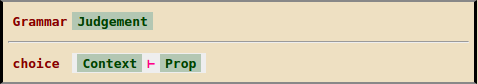
\includegraphics[width=\textwidth]{prop-grammar-judgement}
\end{minipage}
\caption{Definition of \pgmr{Judgement}}
\label{fig:prop-grammar-judgement}
\end{figure}

\newcommand{\propTurnstile}{\pifmt{$\vdash$}}

\pgmr{Judgement} has a meaning of validity. For example, validity of
\term{prop-judgement-ex-1} means, assuming that \term{prop-judgement-ex-1-1} and
\term{prop-judgement-ex-1-2} hold then \term{prop-judgement-ex-1-3} holds.

Please note that \pgmr{Judgement} doesn't have field \kMetaVarRegex nor
\kLiteralRegex \ so we can't accidentally use meta variable or literal for
\pgmr{Judgement}.

\section{Hypothesis rules}

In order to prove any judgement, we want ability to state that for any
proposition that is in assumptions, it can be conclusion i.e. $A_{1..n} \vdash
A_i$ where $i \in {1..n}$

This is achievable by \prule{hypothesis-base} and \prule{hypothesis-next}.

\begin{center}
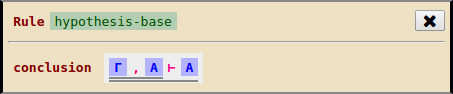
\includegraphics[scale=0.5]{prop-rule-hypo-base}
\end{center}
\begin{center}
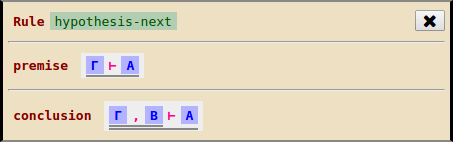
\includegraphics[scale=0.5]{prop-rule-hypo-next}
\end{center}

\prule{hypothesis-base} matches the last assumption with the conclusion whereas
\prule{hypothesis-next} removes the last assumption and pass on to a premise,
this can prove a judgement that has conclusion as assumption like this.

\begin{center}
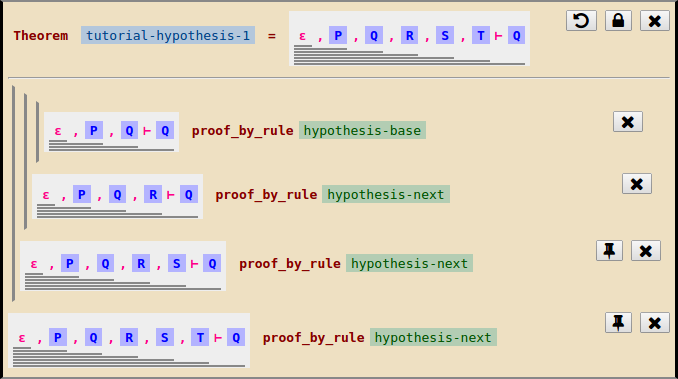
\includegraphics[scale=0.5]{prop-tut-hypo-1}
\end{center}

This is not efficient as we might need to call \prule{hypothesis-next} $(n - 1)$
times where n is the number of assumptions. To solve this problem, we introduce
 \prule{hypothesis} that is more complex than ordinary derivation rule.


\begin{figure}[H]
\begin{minipage}{\textwidth}
    \centering
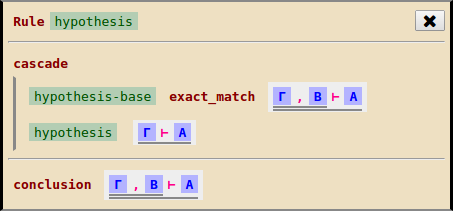
\includegraphics[scale=0.5]{prop-rule-hypo}
\end{minipage}
    \caption{rule \prule{Hypothesis}}
\label{fig:prop-rule-hypothesis}
\end{figure}

\prule{hypothesis} uses a cascade premise instead of direct premise. A cascade
premise has several sub-rules calling-template that will be tried in order. In
this case, \prule{hypothesis} tries to apply \prule{hypothesis-base} on its
goal,
\begin{itemize}
\item If sub-rule is applicable, then use sub-goals generated from sub-rule as
  its sub-goals, in this case, \prule{hypothesis-base} doesn't have any premises
  so this cascade premise has no further sub-goals.
\item Otherwise, \emph{cascade}s down and tries to apply the next sub-rule which
  is \prule{hypothesis} itself\footnote{Yes, it supports recursive call}. Again,
  if applicable, use sub-goals of sub-rule, otherwise, the main
  \prule{hypothesis} rule fail as the cascade premise fail to match with any
  ofsub-rules.
\end{itemize}

\prule{hypothesis} could solve the last theorem like this

\begin{center}
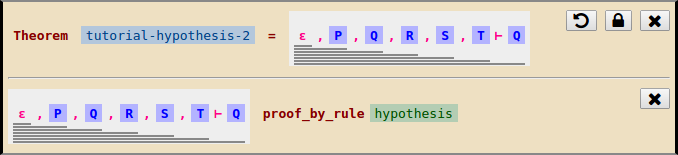
\includegraphics[scale=0.5]{prop-tut-hypo-2}
\end{center}

To show the process, first \prule{hypothesis} conclusion ---
\term{prop-tut-hypo-4} is pattern match against goal = \term{prop-tut-hypo-3},
this results in \pvar{A} = \term{prop-tut-hypo-5}, \pvar{B} =
\term{prop-tut-hypo-6}, and \pvar{$\Gamma$} = \term{prop-tut-hypo-7}. This
cascade premise try to apply \prule{hypothesis-base} with goal\footnote{This is
  result from substitution to that sub-rule goal template. Coincidentally, it is
  the same as \prule{hypothesis} conclusion} = \term{prop-tut-hypo-3}.

\prule{hypothesis-base}, as sub-rule, let \term{prop-tut-hypo-8} pattern match
against \term{prop-tut-hypo-3} and get \pvar{A} = \term{prop-tut-hypo-5},
\pvar{A} = \term{prop-tut-hypo-6}, and \pvar{$\Gamma$} = \term{prop-tut-hypo-7}.
When a meta variable is matched with two or more terms, those terms will be
unified to make pattern match still possible. So \term{prop-tut-hypo-6} will be
replaced by \term{prop-tut-hypo-5} and this sub-rule will success. Here is the
same result if \prule{hypothesis-base} is applied directly on the theorem.

\begin{center}
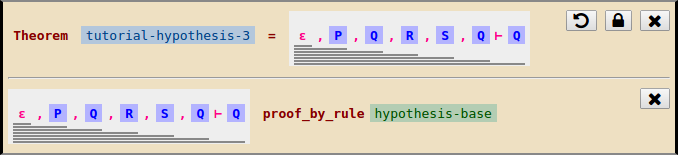
\includegraphics[scale=0.5]{prop-tut-hypo-9}
\end{center}

However, this is not what we want, to avoid this problem, we cat put flag
\kExactMatch\ to this sub-rule, this flag will prevent further unification. Now,
\term{prop-tut-hypo-6} cannot unify with \term{prop-tut-hypo-5} so this sub-rule
fail. So, the cascade premise will move to second sub-rule and try to apply
\prule{hypothesis} with \term{prop-tut-hypo-10}.

\prule{hypothesis}, as sub-rule, let \term{prop-tut-hypo-4} pattern match
against \term{prop-tut-hypo-10}, the process is similar as before so I can tell
directly that it will apply \prule{hypothesis} as sub-sub-rule with goal =
\term{prop-tut-hypo-11}, which in tern, apply \prule{hypothesis} as
sub-sub-sub-rule with goal = \term{prop-tut-hypo-12}.

Now, \prule{hypothesis-base} with goal = \term{prop-tut-hypo-12} will not fail
again since the last assumption and the conclusion is exactly match, i.e. no
further unification needed hence it will success and return no sub-goals as
\prule{hypothesis-base} doesn't have any. This success will propagate up to the
top level and the entire will cascade success with no further sub-goals as shown
in \pthm{tutorial-hypothesis-2}.

Please note that a cascade premise is just another type of a premise, sub-goals
that are generated from sub-rule will replace the cascade premise itself,
similar to how a sub-goal replaces direct premise. Thus, cascade premise can be
used alongside with direct premises, for more information on cascade blocks
please see \hyperref[chap:specification]{specification chapter}.

\hspace{2ex}

\section{Main Rules}

Now, Propositional Logic is ready for new rules as the following,

\begin{figure}[H]
    \centering

\begin{minipage}{0.48\textwidth}
\begin{flushleft}
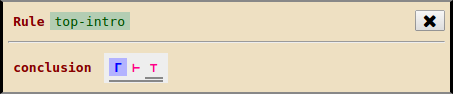
\includegraphics[width=\textwidth]{prop-rule-the-rest-1}
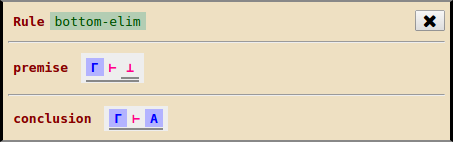
\includegraphics[width=\textwidth]{prop-rule-the-rest-2}
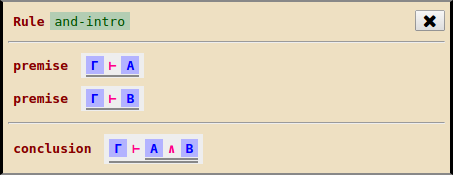
\includegraphics[width=\textwidth]{prop-rule-the-rest-3}
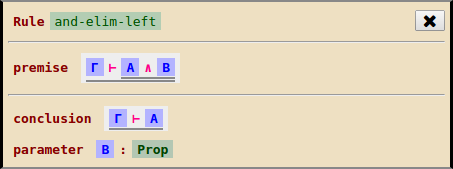
\includegraphics[width=\textwidth]{prop-rule-the-rest-4}
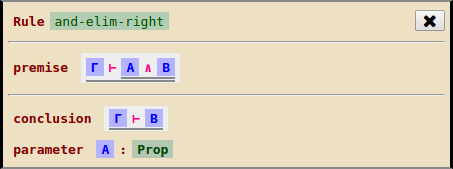
\includegraphics[width=\textwidth]{prop-rule-the-rest-5}
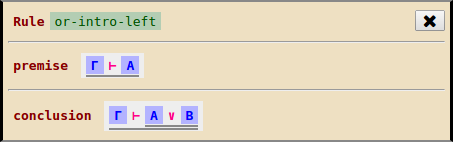
\includegraphics[width=\textwidth]{prop-rule-the-rest-6}
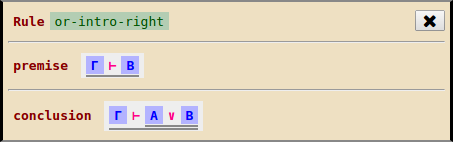
\includegraphics[width=\textwidth]{prop-rule-the-rest-7}
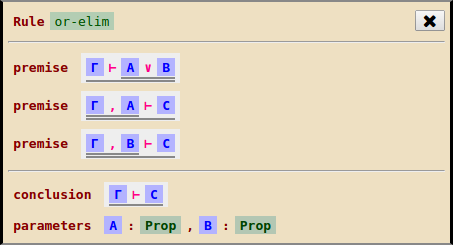
\includegraphics[width=\textwidth]{prop-rule-the-rest-8}
\end{flushleft}
\end{minipage}
~
\begin{minipage}{0.48\textwidth}
\begin{flushright}
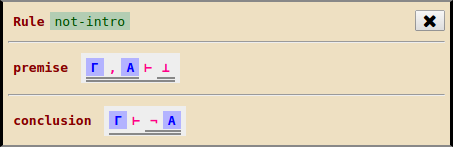
\includegraphics[width=\textwidth]{prop-rule-the-rest-9}
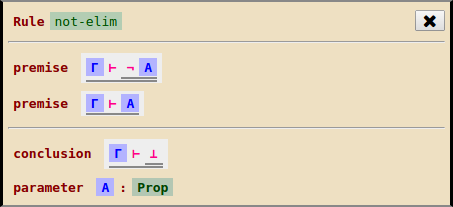
\includegraphics[width=\textwidth]{prop-rule-the-rest-10}
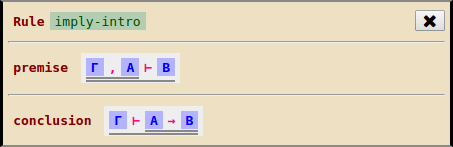
\includegraphics[width=\textwidth]{prop-rule-the-rest-11}
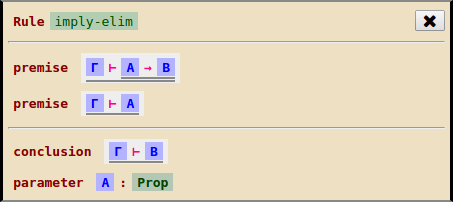
\includegraphics[width=\textwidth]{prop-rule-the-rest-12}
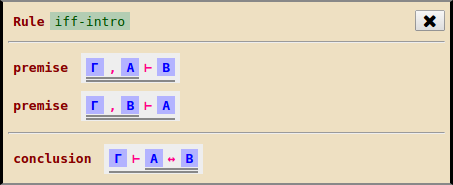
\includegraphics[width=\textwidth]{prop-rule-the-rest-13}
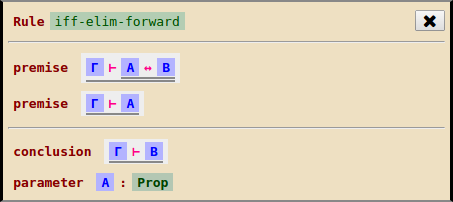
\includegraphics[width=\textwidth]{prop-rule-the-rest-14}
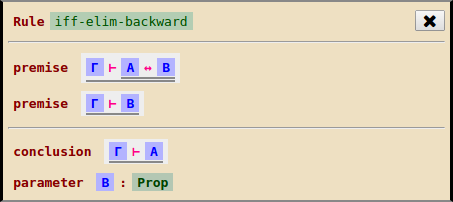
\includegraphics[width=\textwidth]{prop-rule-the-rest-15}
\end{flushright}
\end{minipage}

    \caption{Main Rules for Propositional Logic}
\label{fig:prop-rule-main-rules}
\end{figure}

For example, these rules can be used together with \prule{hypothesis} as the
following

\begin{center}
  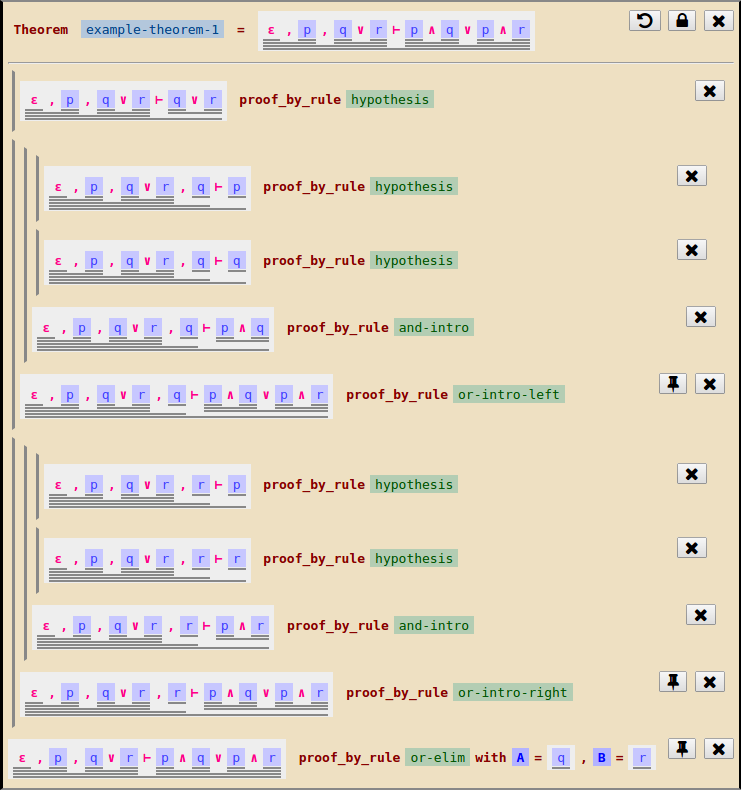
\includegraphics[scale=0.4]{prop-ex-thm-1}
\end{center}
\begin{center}
  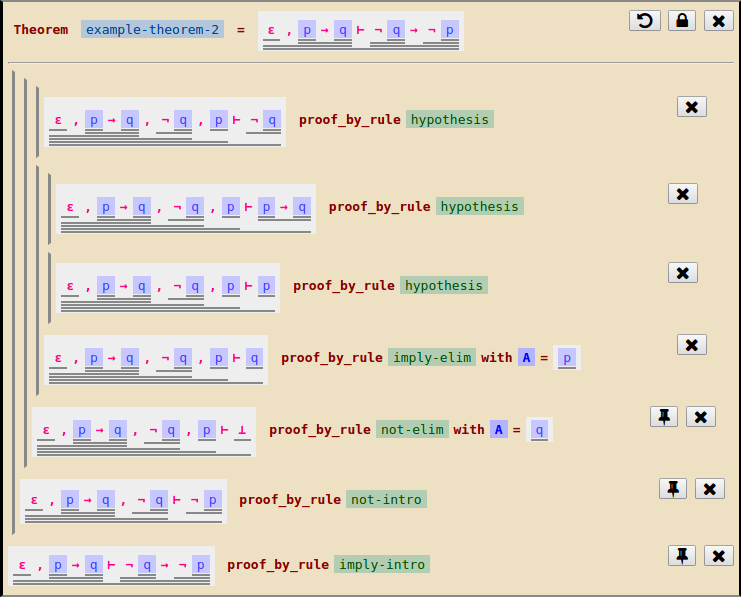
\includegraphics[scale=0.4]{prop-ex-thm-2}
\end{center}

\section{Classical Logic}

The rules so far create Intuitionistic Logic i.e.\ it doesn't assume that each
proposition must be either true or false. Hence, cannot prove some thing like
\term{prop-term-lem-big-a}.

We can introduce rule \prule{proof-by-contradiction}, which is equivalent to
axiom \prule{law-of-exclude-middle} or \prule{double-negation-elim}, to make
Intuitionistic Logic become Classical one.

\begin{center}
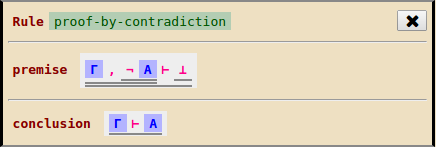
\includegraphics[scale=0.4]{prop-rule-the-rest-16}
\end{center}

And now we can prove \pthm{law-of-exclude-middle} and
\pthm{double-negation-elim} as lemmas.

\begin{center}
  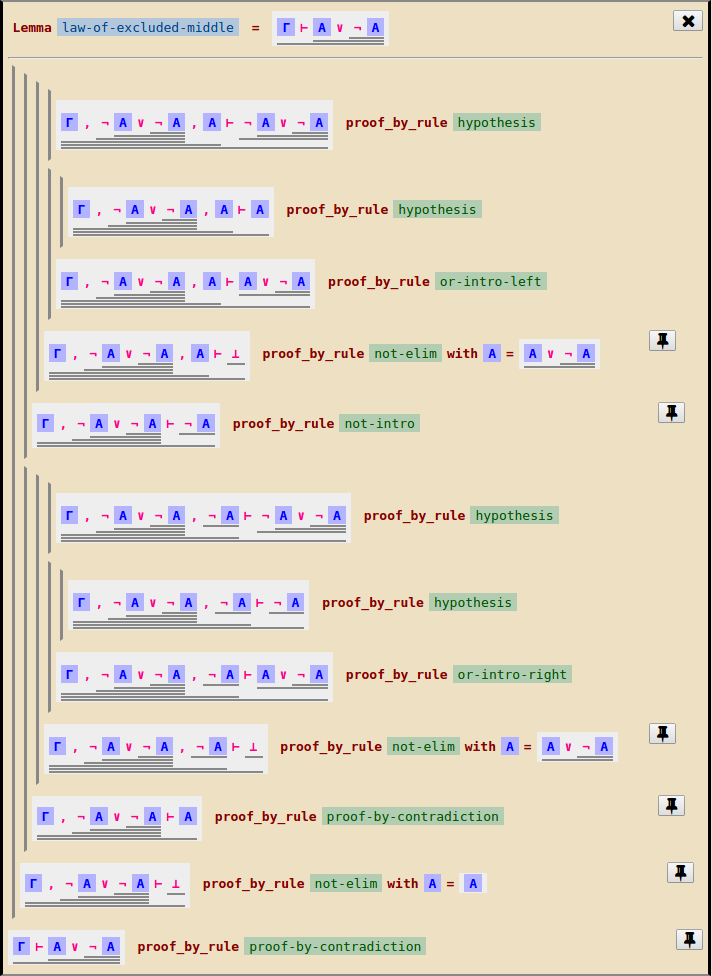
\includegraphics[scale=0.4]{prop-law-of-excluded-middle}
\end{center}

\begin{center}
  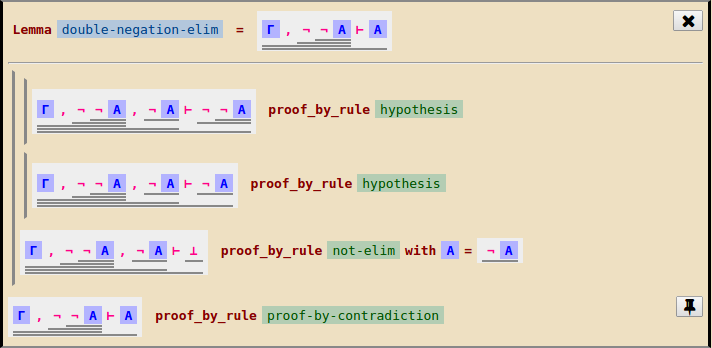
\includegraphics[scale=0.4]{prop-double-negation-elim}
\end{center}

\hspace{1ex}

For example, this example only holds only under Classical Logic.

\hspace{1ex}

\begin{center}
  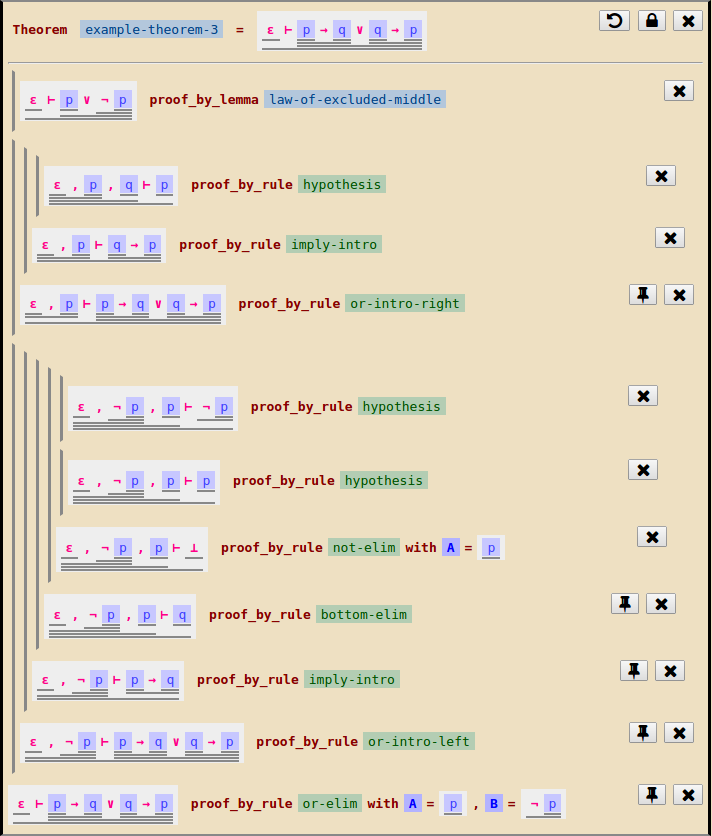
\includegraphics[scale=0.4]{prop-ex-thm-3}
\end{center}

\newpage

\section{Validity of Proposition}
\label{sec:validity_of_proposition}

Although we prove validity of \pgmr{Judgement} to show that a certain proposition
holds under certain assumptions. But \pgmr{Prop} it self has meaning of validity
as well, that is, a proposition holds without any assumptions. The following
rules allow us to prove that a \pgmr{Prop} is valid and make use of its validity
when needed.

\begin{figure}[H]
    \centering


\begin{minipage}{0.48\textwidth}
\begin{flushleft}
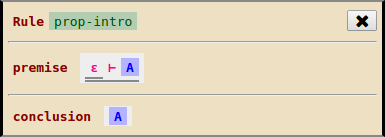
\includegraphics[width=\textwidth]{prop-rule-prop-intro}
\end{flushleft}
\end{minipage}
~
\begin{minipage}{0.48\textwidth}
\begin{flushright}
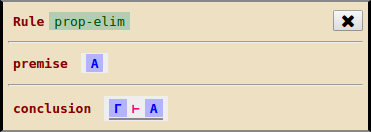
\includegraphics[width=\textwidth]{prop-rule-prop-elim}
\end{flushright}
\end{minipage}

\caption{\prule{prop-intro} can be used to prove that a \pgmr{Prop} is valid.
  And its duality, \prule{prop-elim} can be used to prove \pgmr{Judgement} when
  its conclusion is valid.}
\label{fig:prop-rule-prop-intro-elim}
\end{figure}

For example, the following theorem shows that \term{prop-ex-thm-4-term} always holds
no matter of what \pvar{A} or \pvar{B} will be. Please note that the goal of
this theorem is \pgmr{Prop} rather than \pgmr{Judgement} as usual.

\begin{center}
  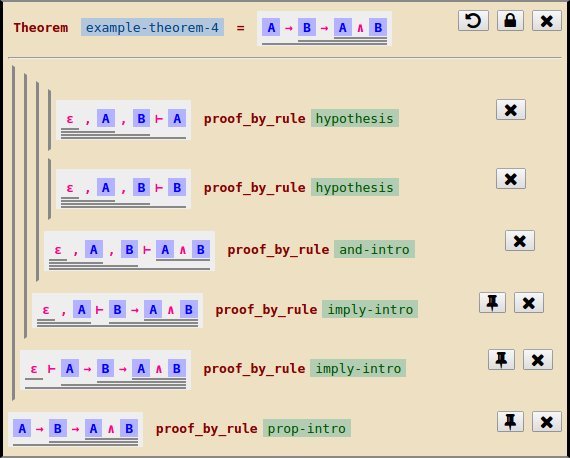
\includegraphics[scale=0.6]{prop-ex-thm-4}
\end{center}

\section{Context manipulation}

Context in Propositional Logic is just a set of assumption so the order and
duplication among assumptions shouldn't matter. Formally, \term{prop-ctx-man-1}
is \emph{definitionally equal} to \term{prop-ctx-man-2} and
\term{prop-ctx-man-3} is \emph{definitionally equal} to
\term{prop-ctx-man-4}. Definitional equality is stronger than object level
equality in the sense that two terms can be equal \emph{implicitly} i.e.\
one term can be transformed to another without any rule or lemma required.

To handle definitional equality, phometa has a mechanism called meta-reduction
which allow a rule that has flag \kAllowReduction\ and doesn't have any
parameters to digest the target term, if it returns exactly one sub-goal that
has the same grammar and doesn't have any further unification, then replace that
sub-goal on the term.

Meta-reduction for context manipulation can be encoded by the following three
rules

\begin{figure}[H]
    \centering

\begin{minipage}{0.48\textwidth}
\begin{flushleft}
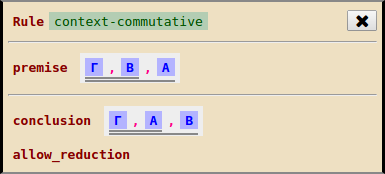
\includegraphics[width=\textwidth]{prop-context-comm}
\end{flushleft}
\end{minipage}
~
\begin{minipage}{0.48\textwidth}
\begin{flushright}
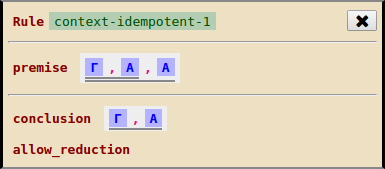
\includegraphics[width=\textwidth]{prop-context-idem-1}
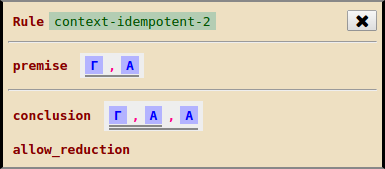
\includegraphics[width=\textwidth]{prop-context-idem-2}
\end{flushright}
\end{minipage}

\caption{Rules for context manipulation}
\label{fig:prop-context-manipulation}
\end{figure}

For example, let construct an unfinished theorem as the following

\begin{center}
  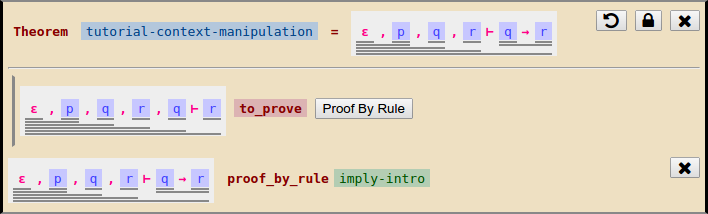
\includegraphics[scale=0.5]{prop-ctx-man-5}
\end{center}

Then, if you click \term{prop-ctx-man-6} on the sub-goal, the keymap will look
like this

\begin{center}
  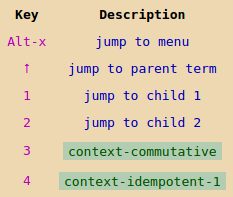
\includegraphics[scale=0.5]{prop-ctx-man-7}
\end{center}

Keymap says that this term is reducible by either \prule{context-commutative} or \\
\prule{context-idempotent-1}. Now we will swap the last two assumption by
pressing \pkbd{4} or clicking the row the keymap directly, the theorem will look
like this.

\begin{center}
  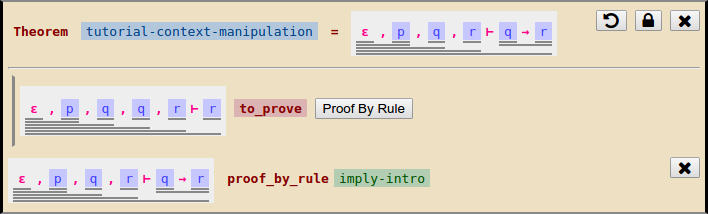
\includegraphics[scale=0.5]{prop-ctx-man-8}
\end{center}

We want to eliminate duplication on of \term{prop-ctx-man-9}, this canbe
done by clicking \term{prop-ctx-man-10} \\ now \prule{context-idempotent-2} is also
available in keymap so we can select it.

\begin{center}
  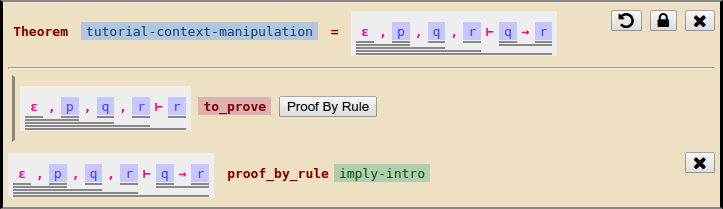
\includegraphics[scale=0.5]{prop-ctx-man-11}
\end{center}

Although I said that white background means not modifiable, but meta-reduction
is exceptional because its implicitness. Meta-reduction is very powerful but
also dangerous so I limit usage of meta-reduction only for \emph{empty}
sub-goal\footnote{Sub-goal that has associate lemma or rule (including the one
  that is waiting for parameter(s)), is not empty sub-goal.} in unfinished
theorem where proving process will benefit from it. In contrast, it doesn't make
sense to do this in rules or lemmas and only make user confuse.

Context manipulation is not that important to for Propositional Logic since rule
\prule{hypothesis} can penetrate thought out of \pgmr{Context}. However, is
better to show it here so you will know how meta-reduction works. This is
particularly important when we start to implement Lambda Calculus in the next
chapter.

\section{How to build Grammars and Rules}
\label{sec:how_to_built_grammars_and_rules}

So far we introduce grammars and rules out of the box, this allows user to prove
a theorem which is the most important part directly. However, Phometa also have
ability to create new grammars and rules as well.

To show how to build these, I will recreate \pgmr{Prop} for grammars and
recreate \prule{or-elim} and \prule{hypothesis} for rules.

\subsection{Recreation of \pgmr{Prop}}

The first step, we need to press ``Add Grammar'' on one of adding panels in
module ``Propositional Logic'', then enter the grammar name. I will use
``TutorialProp'' to avoid conflict with the real one.

\begin{center}
  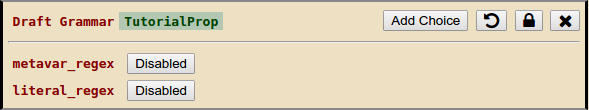
\includegraphics[scale=0.5]{prop-tut-prop-1}
\end{center}

This is just a draft grammar i.e.\ it cannot be used by any rule or any theorem
at the moment. To specify regular expression for meta variable, click a button
that follow \kMetaVarRegex, the button will tern to input box so you can write
regular expression\footnote{Please note that this regular expression must comply to
JavaScript regexp specification.} here,

\begin{center}
  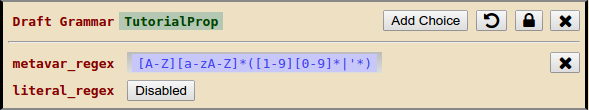
\includegraphics[scale=0.5]{prop-tut-prop-2}
\end{center}

The background colour of this regular expression is grey, so you can edit it
afterword by click the box again. Alternatively you can delete it using close
button on the right of the row.

For \kLiteralRegex, we do nothing about it as \pgmr{TutorialProp} will not
instantiate literal.

Next, we will add choices to the grammar, I will start with the one that has
``$\wedge$'' connector. Click ``Add Choice'' button on the header of this
grammar, it will tern to be input box that you can write number of sub-grammars
for this choice, in this case it is 2, so write it and press enter.

\begin{center}
  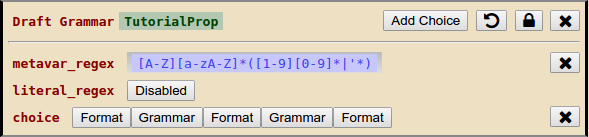
\includegraphics[scale=0.5]{prop-tut-prop-3}
\end{center}

You will see a \kChoice\ that have buttons labelled ``Grammar'', you can
click it to specify a sub-grammar. In this case, select \pgmr{TutorialProp} in
both of position.

There are other three buttons labelled ``Format'' intersperse sub-grammars which
accept any string that will be used as syntax, you can also use unicode input
method similar when we construct a term in last chapter. In this case, click
button in the middle, press \pkbd{Alt-u}, and type ``wedge'', you will see
``$\wedge$'' on the keymap pane, then click it. ``$\wedge$'' will appear in
input box of middle ``Format''. Then hit \pkbd{Return} to finished writing this.

\begin{center}
  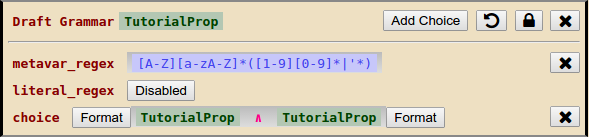
\includegraphics[scale=0.5]{prop-tut-prop-4}
\end{center}

The background colour of these are gray so you can edit it similar to
\kMetaVarRegex. For the first and last ``Format'' buttons, we do nothing on it
as this choice make no use on those positions.

Other choices can be done in similar way, once you finish adding choices, it
should look like this.

\begin{center}
  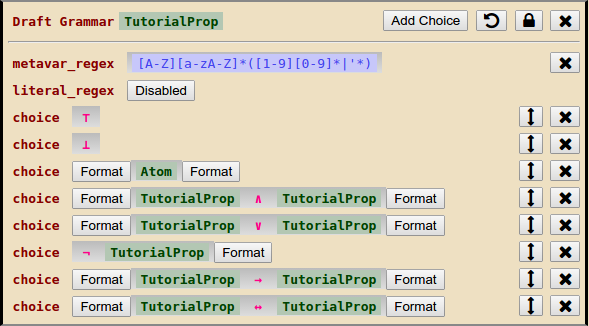
\includegraphics[scale=0.5]{prop-tut-prop-5}
\end{center}

You can lock this draft grammar by clicking lock button on top-right corner,
this will transform it as a proper grammar where you can refer it in rules and
theorems.

\begin{center}
  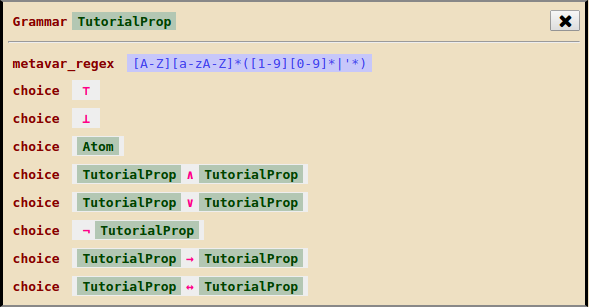
\includegraphics[scale=0.5]{prop-tut-prop-6}
\end{center}

\subsection{Recreation of \prule{or-elim}}

The next thing that we recreate is rule \prule{or-elim}. First, click ``Add
Rule'' in adding panel and write ``tutorial-or-elim'' on it.

\begin{center}
  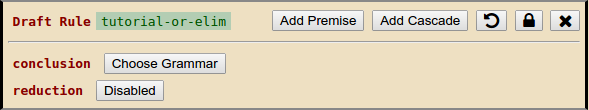
\includegraphics[scale=0.5]{prop-tut-or-elim-1}
\end{center}

This is just a draft rule i.e.\ it cannot be used by any theorem at the moment.
Let start by filling \kConclusion, we just need to input a term similar to when
we input a goal of a theorem.

\begin{center}
  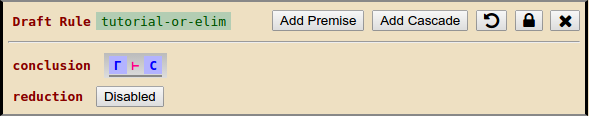
\includegraphics[scale=0.5]{prop-tut-or-elim-2}
\end{center}

Next is \kAllowReduction\, it is disabled by default, we could click on button
``Disable'' to toggle it to ``Enable'', however, we don't want to rise this flag
for \prule{tutorial-or-elim} so leave it as it is.

Now, let build the first \kPremise\ by clicking ``Add Premise'' on the top-right
corner of this rule.

\begin{center}
  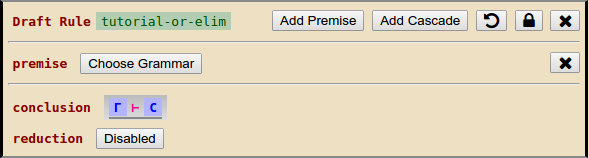
\includegraphics[scale=0.5]{prop-tut-or-elim-3}
\end{center}

Then write a term similar to what we have done in \kConclusion\

\begin{center}
  \includegraphics[scale=0.5]{prop-tut-or-elim-4}
\end{center}

You can see that there is \kParameter\ row pop-up. This represents meta
variables that appear in one of \kPremise\ but not in \kConclusion\ and you can't
manually change it.

The two remaining premises can be done by similar process above

\begin{center}
  \includegraphics[scale=0.5]{prop-tut-or-elim-5}
\end{center}

You can lock this draft rule by clicking lock button on top-right corner,
this will transform it as a proper rule where you can refer it in theorems.

\begin{center}
  \includegraphics[scale=0.5]{prop-tut-or-elim-6}
\end{center}

\newpage

\subsection{Recreation of \prule{hypothesis}}

The recreation of \prule{or-elim} shows most of features of rule construction
except how to deal with cascade so we will recreate \prule{hypothesis} to
illustrate this. First, adding a rule with name ``tutorial-hypothesis'' on it.
Then, enter a term for \kConclusion.

\begin{center}
  \includegraphics[scale=0.5]{prop-tut-rule-hypo-1}
\end{center}

Then, add a cascade premise by clicking ``Add Cascade'' on the top-right corner.

\begin{center}
  \includegraphics[scale=0.5]{prop-tut-rule-hypo-2}
\end{center}

Then click ``Add Sub-Rule'' to add the first sub-rule, the button will
transformed into input box where you can select such a rule, in this case select
\prule{hypothesis-base}

\begin{center}
  \includegraphics[scale=0.5]{prop-tut-rule-hypo-3}
\end{center}

Sub-rule calling-template will appear, you can construct a term that will passed
into this sub-rule. A sub-rule is unifiable by default, you can set it to
\kExactMatch\ by toggling button ``Unifiable''.

\begin{center}
  \includegraphics[scale=0.5]{prop-tut-rule-hypo-4}
\end{center}

The second sub-rule could be construct on similar manner to the first one.

\begin{center}
  \includegraphics[scale=0.5]{prop-tut-rule-hypo-5}
\end{center}

Then you can lock this draft rule, to change it to a proper rule.

\begin{center}
  \includegraphics[scale=0.5]{prop-tut-rule-hypo-6}
\end{center}

\newpage

\section{Exercises}

Credit: Some of material here modified from tutorial 3, 4, and 5 of first year Logic
course, Department of Computing, Imperial College London. Thank you Prof Ian
Hodkinson and Dr Krysia Broda for this.

\begin{itemize}
\item Create a theorem and proof each of the following
  \begin{itemize}
  \item \term{prop-ex-1-a}
  \item \term{prop-ex-1-b} (reminder: this is \pgmr{Prop} not \pgmr{Judgement})
  \item \term{prop-ex-1-c}
  \item \term{prop-ex-1-d}
  \item \term{prop-ex-1-e}
  \item \term{prop-ex-1-f}
  \item \term{prop-ex-1-g}
  \item \term{prop-ex-2-a}
  \item \term{prop-ex-2-b}
  \item \term{prop-ex-2-c}
  \item \term{prop-ex-2-d}
  \item \term{prop-ex-2-e}
  \item \term{prop-ex-2-f}
  \item \term{prop-ex-2-g}
  \item \term{prop-ex-2-h}
  \item \term{prop-ex-2-i}
  \item \term{prop-ex-2-j}
  \end{itemize}
\item Equivalence of Propositional Logic could be written in the form ($A \equiv
  B$) stated that, $A$ holds if and only if $B$ holds. Please
  introduce new a grammar \pgmr{Equivalence} and write \prule{equiv-intro}
  similar section \ref{sec:validity_of_proposition} and prove the following
  \begin{itemize}
  \item \term{prop-ex-eqv-1}
  \item \term{prop-ex-eqv-2}
  \item \term{prop-ex-eqv-3}
  \item \term{prop-ex-eqv-4}
  \item \term{prop-ex-eqv-5}
  \item \term{prop-ex-eqv-6}
  \item \term{prop-ex-eqv-7}
  \item \term{prop-ex-eqv-8}
  \item \term{prop-ex-eqv-9}
  \item \term{prop-ex-eqv-10}
  \item \term{prop-ex-eqv-11}
  \item \term{prop-ex-eqv-12}
  \item \term{prop-ex-eqv-13}
  \item \term{prop-ex-eqv-14}
  \item \term{prop-ex-eqv-15}
  \end{itemize}
\item (Challenge) Extend this Propositional Logic to become First Order Logic.
\end{itemize}

\end{document}